% Fig. 3.10 -- 三個變數依序遞增且都小於 u 所對應的區域: 縮小的四面體。
% 書稿來源: mathstatch3.tex 第 1041 行的 tikzpicture (scale=.7)。
%
% 幾何一律照書稿: 結構與 Fig. 3.9 相同 (view={320}{345}、三軸標 $x_1$、$x_2$、$x_3$)，
% 差別有二: 三軸的刻度改為 0、0.5、u、1 (書稿以 0.7 代表 u 的位置)；
% 四面體縮到以 (0,0,0)、(0,0,u)、(0,u,u) 與 (u,u,u) 為頂點。
% 輔助虛線也與 Fig. 3.9 不同: 共用的只有 (x,x,x)、(0,x,x) 與 (x,x,1) 三條，
% 另加 (x,u,u)、(x,x,u) 與 (0,x,u) 三條只畫到 u 為止的虛線。
%
% 對書稿的四處調整同 Fig. 3.9:
%   1. 填色由 gray 0.2 改為 journalaccent 0.15；虛線改 journalmuted 0.5pt、
%      實線與座標軸改 journalink 0.8pt。
%   2. 不以 scale=.7 縮圖，改為直接指定 axis 的 width，並以 \DeclareMathSizes
%      把 script 級撐到 9pt。
%   3. 以 xmin/xmax/ymin/ymax 與 enlargelimits=false 取代書稿末尾那道
%      opacity=0 的 \addplot3[surf]，成圖相同而路徑數大減。
%   4. 本圖置於 Example 方框之內，手機顯示寬為 309px 而非 350px，字級依 309px 核算。
%
% 量測: viewBox 寬 216.67pt，309px 之下放大 1.4261 倍，最小字 9pt 折合 12.83px
%       (350px 之下為 14.54px)。成圖 17 KB，gzip 之後 5.5 KB，路徑 44 條。
%
% 產製 (CH3 規格 3.2 的 pgfplots 路徑，-O 不可省):
%   latex -interaction=nonstopmode '\def\pgfsysdriver{pgfsys-dvisvgm.def}% Fig. 3.10 -- 三個變數依序遞增且都小於 u 所對應的區域: 縮小的四面體。
% 書稿來源: mathstatch3.tex 第 1041 行的 tikzpicture (scale=.7)。
%
% 幾何一律照書稿: 結構與 Fig. 3.9 相同 (view={320}{345}、三軸標 $x_1$、$x_2$、$x_3$)，
% 差別有二: 三軸的刻度改為 0、0.5、u、1 (書稿以 0.7 代表 u 的位置)；
% 四面體縮到以 (0,0,0)、(0,0,u)、(0,u,u) 與 (u,u,u) 為頂點。
% 輔助虛線也與 Fig. 3.9 不同: 共用的只有 (x,x,x)、(0,x,x) 與 (x,x,1) 三條，
% 另加 (x,u,u)、(x,x,u) 與 (0,x,u) 三條只畫到 u 為止的虛線。
%
% 對書稿的四處調整同 Fig. 3.9:
%   1. 填色由 gray 0.2 改為 journalaccent 0.15；虛線改 journalmuted 0.5pt、
%      實線與座標軸改 journalink 0.8pt。
%   2. 不以 scale=.7 縮圖，改為直接指定 axis 的 width，並以 \DeclareMathSizes
%      把 script 級撐到 9pt。
%   3. 以 xmin/xmax/ymin/ymax 與 enlargelimits=false 取代書稿末尾那道
%      opacity=0 的 \addplot3[surf]，成圖相同而路徑數大減。
%   4. 本圖置於 Example 方框之內，手機顯示寬為 309px 而非 350px，字級依 309px 核算。
%
% 量測: viewBox 寬 216.67pt，309px 之下放大 1.4261 倍，最小字 9pt 折合 12.83px
%       (350px 之下為 14.54px)。成圖 17 KB，gzip 之後 5.5 KB，路徑 44 條。
%
% 產製 (CH3 規格 3.2 的 pgfplots 路徑，-O 不可省):
%   latex -interaction=nonstopmode '\def\pgfsysdriver{pgfsys-dvisvgm.def}% Fig. 3.10 -- 三個變數依序遞增且都小於 u 所對應的區域: 縮小的四面體。
% 書稿來源: mathstatch3.tex 第 1041 行的 tikzpicture (scale=.7)。
%
% 幾何一律照書稿: 結構與 Fig. 3.9 相同 (view={320}{345}、三軸標 $x_1$、$x_2$、$x_3$)，
% 差別有二: 三軸的刻度改為 0、0.5、u、1 (書稿以 0.7 代表 u 的位置)；
% 四面體縮到以 (0,0,0)、(0,0,u)、(0,u,u) 與 (u,u,u) 為頂點。
% 輔助虛線也與 Fig. 3.9 不同: 共用的只有 (x,x,x)、(0,x,x) 與 (x,x,1) 三條，
% 另加 (x,u,u)、(x,x,u) 與 (0,x,u) 三條只畫到 u 為止的虛線。
%
% 對書稿的四處調整同 Fig. 3.9:
%   1. 填色由 gray 0.2 改為 journalaccent 0.15；虛線改 journalmuted 0.5pt、
%      實線與座標軸改 journalink 0.8pt。
%   2. 不以 scale=.7 縮圖，改為直接指定 axis 的 width，並以 \DeclareMathSizes
%      把 script 級撐到 9pt。
%   3. 以 xmin/xmax/ymin/ymax 與 enlargelimits=false 取代書稿末尾那道
%      opacity=0 的 \addplot3[surf]，成圖相同而路徑數大減。
%   4. 本圖置於 Example 方框之內，手機顯示寬為 309px 而非 350px，字級依 309px 核算。
%
% 量測: viewBox 寬 216.67pt，309px 之下放大 1.4261 倍，最小字 9pt 折合 12.83px
%       (350px 之下為 14.54px)。成圖 17 KB，gzip 之後 5.5 KB，路徑 44 條。
%
% 產製 (CH3 規格 3.2 的 pgfplots 路徑，-O 不可省):
%   latex -interaction=nonstopmode '\def\pgfsysdriver{pgfsys-dvisvgm.def}% Fig. 3.10 -- 三個變數依序遞增且都小於 u 所對應的區域: 縮小的四面體。
% 書稿來源: mathstatch3.tex 第 1041 行的 tikzpicture (scale=.7)。
%
% 幾何一律照書稿: 結構與 Fig. 3.9 相同 (view={320}{345}、三軸標 $x_1$、$x_2$、$x_3$)，
% 差別有二: 三軸的刻度改為 0、0.5、u、1 (書稿以 0.7 代表 u 的位置)；
% 四面體縮到以 (0,0,0)、(0,0,u)、(0,u,u) 與 (u,u,u) 為頂點。
% 輔助虛線也與 Fig. 3.9 不同: 共用的只有 (x,x,x)、(0,x,x) 與 (x,x,1) 三條，
% 另加 (x,u,u)、(x,x,u) 與 (0,x,u) 三條只畫到 u 為止的虛線。
%
% 對書稿的四處調整同 Fig. 3.9:
%   1. 填色由 gray 0.2 改為 journalaccent 0.15；虛線改 journalmuted 0.5pt、
%      實線與座標軸改 journalink 0.8pt。
%   2. 不以 scale=.7 縮圖，改為直接指定 axis 的 width，並以 \DeclareMathSizes
%      把 script 級撐到 9pt。
%   3. 以 xmin/xmax/ymin/ymax 與 enlargelimits=false 取代書稿末尾那道
%      opacity=0 的 \addplot3[surf]，成圖相同而路徑數大減。
%   4. 本圖置於 Example 方框之內，手機顯示寬為 309px 而非 350px，字級依 309px 核算。
%
% 量測: viewBox 寬 216.67pt，309px 之下放大 1.4261 倍，最小字 9pt 折合 12.83px
%       (350px 之下為 14.54px)。成圖 17 KB，gzip 之後 5.5 KB，路徑 44 條。
%
% 產製 (CH3 規格 3.2 的 pgfplots 路徑，-O 不可省):
%   latex -interaction=nonstopmode '\def\pgfsysdriver{pgfsys-dvisvgm.def}\input{three-uniform-region-b.tex}'
%   dvisvgm -O -d2 -n -o ../../images/teaching-topics/three-uniform-region-b.svg three-uniform-region-b.dvi

\documentclass[tikz,border=2pt]{standalone}
\usepackage{amsmath}
\usepackage{amssymb}
\usepackage{xcolor}
\usepackage{pgfplots}
\pgfplotsset{compat=1.18}

\definecolor{journalink}{HTML}{1F1C18}
\definecolor{journalmuted}{HTML}{8A7F72}
\definecolor{journalaccent}{HTML}{9C2D2D}

%% 三個軸名的下標一律撐到 9pt。
\DeclareMathSizes{10}{10}{9}{8}

\begin{document}
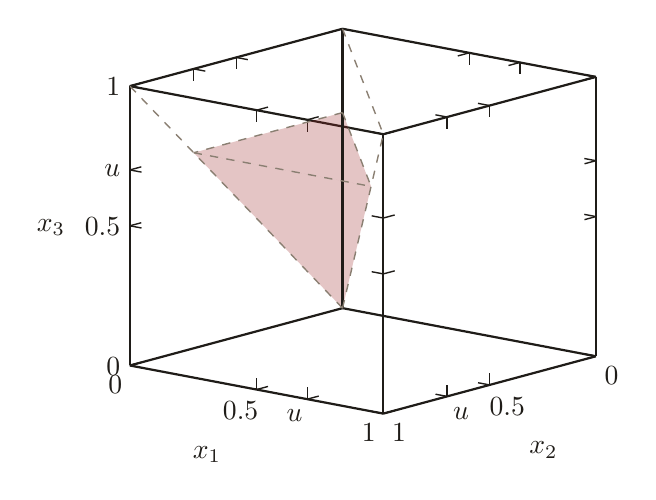
\begin{tikzpicture}
\begin{axis}[
    width=7.5cm,
    view={320}{345},
    xlabel=$x_1$,
    ylabel={$x_2$},
    zlabel={$x_3$},
    zlabel style={rotate=-90, anchor=east},
    label style={journalink},
    tick label style={journalink},
    axis line style={journalink, line width=0.8pt},
    every tick/.style={journalink, line width=0.5pt},
    enlargelimits=false,
    xmin=0, xmax=1,
    ymin=0, ymax=1,
    zmin=0, zmax=1,
    xtick={0,0.5,0.7,1}, xticklabels={0,0.5,$u$,1},
    ytick={0,0.5,0.7,1}, yticklabels={0,0.5,$u$,1},
    ztick={0,0.5,0.7,1}, zticklabels={0,0.5,$u$,1},
]

%% 四面體的四個面
\fill[journalaccent, fill opacity=0.15]
  (axis cs: 0,0,0) -- (axis cs: 0,0,0.7) -- (axis cs: 0,0.7,0.7) -- cycle;
\fill[journalaccent, fill opacity=0.15]
  (axis cs: 0,0,0) -- (axis cs: 0,0,0.7) -- (axis cs: 0.7,0.7,0.7) -- cycle;
\fill[journalaccent, fill opacity=0.15]
  (axis cs: 0,0,0) -- (axis cs: 0,0.7,0.7) -- (axis cs: 0.7,0.7,0.7) -- cycle;
\fill[journalaccent, fill opacity=0.15]
  (axis cs: 0,0,0.7) -- (axis cs: 0,0.7,0.7) -- (axis cs: 0.7,0.7,0.7) -- cycle;

%% 立方體靠前的三條稜邊
\addplot3 [journalink, line width=0.8pt, domain=0:1, samples y=1, smooth] (0, 0, x);
\addplot3 [journalink, line width=0.8pt, domain=0:1, samples y=1, smooth] (0, x, 0);
\addplot3 [journalink, line width=0.8pt, domain=0:1, samples y=1, smooth] (x, 0, 0);

%% 六條輔助虛線
\addplot3 [journalmuted, line width=0.5pt, dashed, domain=0:1, samples y=1, smooth] (x, x, x);
\addplot3 [journalmuted, line width=0.5pt, dashed, domain=0:1, samples y=1, smooth] (0, x, x);
\addplot3 [journalmuted, line width=0.5pt, dashed, domain=0:0.7, samples y=1, smooth] (x, 0.7, 0.7);
\addplot3 [journalmuted, line width=0.5pt, dashed, domain=0:0.7, samples y=1, smooth] (x, x, 0.7);
\addplot3 [journalmuted, line width=0.5pt, dashed, domain=0:1, samples y=1, smooth] (x, x, 1);
\addplot3 [journalmuted, line width=0.5pt, dashed, domain=0:0.7, samples y=1, smooth] (0, x, 0.7);

\end{axis}
\end{tikzpicture}
\end{document}
'
%   dvisvgm -O -d2 -n -o ../../images/teaching-topics/three-uniform-region-b.svg three-uniform-region-b.dvi

\documentclass[tikz,border=2pt]{standalone}
\usepackage{amsmath}
\usepackage{amssymb}
\usepackage{xcolor}
\usepackage{pgfplots}
\pgfplotsset{compat=1.18}

\definecolor{journalink}{HTML}{1F1C18}
\definecolor{journalmuted}{HTML}{8A7F72}
\definecolor{journalaccent}{HTML}{9C2D2D}

%% 三個軸名的下標一律撐到 9pt。
\DeclareMathSizes{10}{10}{9}{8}

\begin{document}
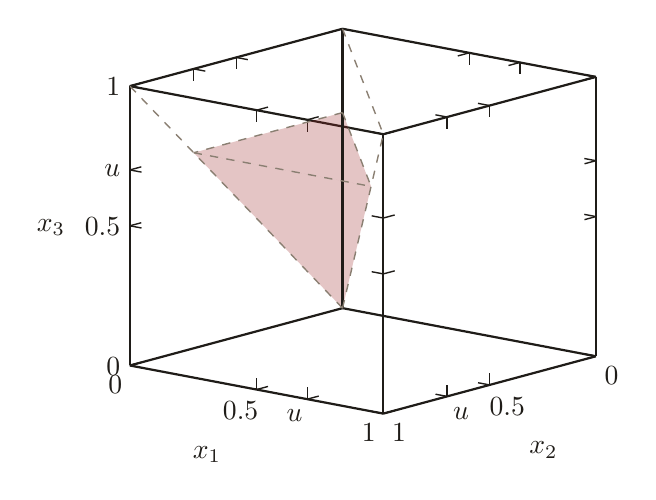
\begin{tikzpicture}
\begin{axis}[
    width=7.5cm,
    view={320}{345},
    xlabel=$x_1$,
    ylabel={$x_2$},
    zlabel={$x_3$},
    zlabel style={rotate=-90, anchor=east},
    label style={journalink},
    tick label style={journalink},
    axis line style={journalink, line width=0.8pt},
    every tick/.style={journalink, line width=0.5pt},
    enlargelimits=false,
    xmin=0, xmax=1,
    ymin=0, ymax=1,
    zmin=0, zmax=1,
    xtick={0,0.5,0.7,1}, xticklabels={0,0.5,$u$,1},
    ytick={0,0.5,0.7,1}, yticklabels={0,0.5,$u$,1},
    ztick={0,0.5,0.7,1}, zticklabels={0,0.5,$u$,1},
]

%% 四面體的四個面
\fill[journalaccent, fill opacity=0.15]
  (axis cs: 0,0,0) -- (axis cs: 0,0,0.7) -- (axis cs: 0,0.7,0.7) -- cycle;
\fill[journalaccent, fill opacity=0.15]
  (axis cs: 0,0,0) -- (axis cs: 0,0,0.7) -- (axis cs: 0.7,0.7,0.7) -- cycle;
\fill[journalaccent, fill opacity=0.15]
  (axis cs: 0,0,0) -- (axis cs: 0,0.7,0.7) -- (axis cs: 0.7,0.7,0.7) -- cycle;
\fill[journalaccent, fill opacity=0.15]
  (axis cs: 0,0,0.7) -- (axis cs: 0,0.7,0.7) -- (axis cs: 0.7,0.7,0.7) -- cycle;

%% 立方體靠前的三條稜邊
\addplot3 [journalink, line width=0.8pt, domain=0:1, samples y=1, smooth] (0, 0, x);
\addplot3 [journalink, line width=0.8pt, domain=0:1, samples y=1, smooth] (0, x, 0);
\addplot3 [journalink, line width=0.8pt, domain=0:1, samples y=1, smooth] (x, 0, 0);

%% 六條輔助虛線
\addplot3 [journalmuted, line width=0.5pt, dashed, domain=0:1, samples y=1, smooth] (x, x, x);
\addplot3 [journalmuted, line width=0.5pt, dashed, domain=0:1, samples y=1, smooth] (0, x, x);
\addplot3 [journalmuted, line width=0.5pt, dashed, domain=0:0.7, samples y=1, smooth] (x, 0.7, 0.7);
\addplot3 [journalmuted, line width=0.5pt, dashed, domain=0:0.7, samples y=1, smooth] (x, x, 0.7);
\addplot3 [journalmuted, line width=0.5pt, dashed, domain=0:1, samples y=1, smooth] (x, x, 1);
\addplot3 [journalmuted, line width=0.5pt, dashed, domain=0:0.7, samples y=1, smooth] (0, x, 0.7);

\end{axis}
\end{tikzpicture}
\end{document}
'
%   dvisvgm -O -d2 -n -o ../../images/teaching-topics/three-uniform-region-b.svg three-uniform-region-b.dvi

\documentclass[tikz,border=2pt]{standalone}
\usepackage{amsmath}
\usepackage{amssymb}
\usepackage{xcolor}
\usepackage{pgfplots}
\pgfplotsset{compat=1.18}

\definecolor{journalink}{HTML}{1F1C18}
\definecolor{journalmuted}{HTML}{8A7F72}
\definecolor{journalaccent}{HTML}{9C2D2D}

%% 三個軸名的下標一律撐到 9pt。
\DeclareMathSizes{10}{10}{9}{8}

\begin{document}
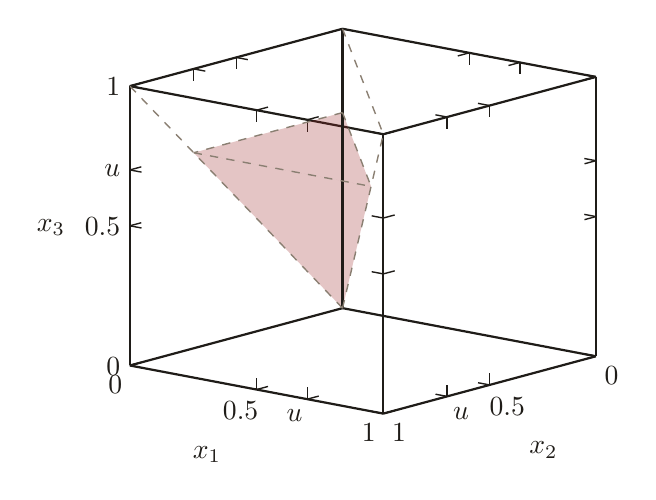
\begin{tikzpicture}
\begin{axis}[
    width=7.5cm,
    view={320}{345},
    xlabel=$x_1$,
    ylabel={$x_2$},
    zlabel={$x_3$},
    zlabel style={rotate=-90, anchor=east},
    label style={journalink},
    tick label style={journalink},
    axis line style={journalink, line width=0.8pt},
    every tick/.style={journalink, line width=0.5pt},
    enlargelimits=false,
    xmin=0, xmax=1,
    ymin=0, ymax=1,
    zmin=0, zmax=1,
    xtick={0,0.5,0.7,1}, xticklabels={0,0.5,$u$,1},
    ytick={0,0.5,0.7,1}, yticklabels={0,0.5,$u$,1},
    ztick={0,0.5,0.7,1}, zticklabels={0,0.5,$u$,1},
]

%% 四面體的四個面
\fill[journalaccent, fill opacity=0.15]
  (axis cs: 0,0,0) -- (axis cs: 0,0,0.7) -- (axis cs: 0,0.7,0.7) -- cycle;
\fill[journalaccent, fill opacity=0.15]
  (axis cs: 0,0,0) -- (axis cs: 0,0,0.7) -- (axis cs: 0.7,0.7,0.7) -- cycle;
\fill[journalaccent, fill opacity=0.15]
  (axis cs: 0,0,0) -- (axis cs: 0,0.7,0.7) -- (axis cs: 0.7,0.7,0.7) -- cycle;
\fill[journalaccent, fill opacity=0.15]
  (axis cs: 0,0,0.7) -- (axis cs: 0,0.7,0.7) -- (axis cs: 0.7,0.7,0.7) -- cycle;

%% 立方體靠前的三條稜邊
\addplot3 [journalink, line width=0.8pt, domain=0:1, samples y=1, smooth] (0, 0, x);
\addplot3 [journalink, line width=0.8pt, domain=0:1, samples y=1, smooth] (0, x, 0);
\addplot3 [journalink, line width=0.8pt, domain=0:1, samples y=1, smooth] (x, 0, 0);

%% 六條輔助虛線
\addplot3 [journalmuted, line width=0.5pt, dashed, domain=0:1, samples y=1, smooth] (x, x, x);
\addplot3 [journalmuted, line width=0.5pt, dashed, domain=0:1, samples y=1, smooth] (0, x, x);
\addplot3 [journalmuted, line width=0.5pt, dashed, domain=0:0.7, samples y=1, smooth] (x, 0.7, 0.7);
\addplot3 [journalmuted, line width=0.5pt, dashed, domain=0:0.7, samples y=1, smooth] (x, x, 0.7);
\addplot3 [journalmuted, line width=0.5pt, dashed, domain=0:1, samples y=1, smooth] (x, x, 1);
\addplot3 [journalmuted, line width=0.5pt, dashed, domain=0:0.7, samples y=1, smooth] (0, x, 0.7);

\end{axis}
\end{tikzpicture}
\end{document}
'
%   dvisvgm -O -d2 -n -o ../../images/teaching-topics/three-uniform-region-b.svg three-uniform-region-b.dvi

\documentclass[tikz,border=2pt]{standalone}
\usepackage{amsmath}
\usepackage{amssymb}
\usepackage{xcolor}
\usepackage{pgfplots}
\pgfplotsset{compat=1.18}

\definecolor{journalink}{HTML}{1F1C18}
\definecolor{journalmuted}{HTML}{8A7F72}
\definecolor{journalaccent}{HTML}{9C2D2D}

%% 三個軸名的下標一律撐到 9pt。
\DeclareMathSizes{10}{10}{9}{8}

\begin{document}
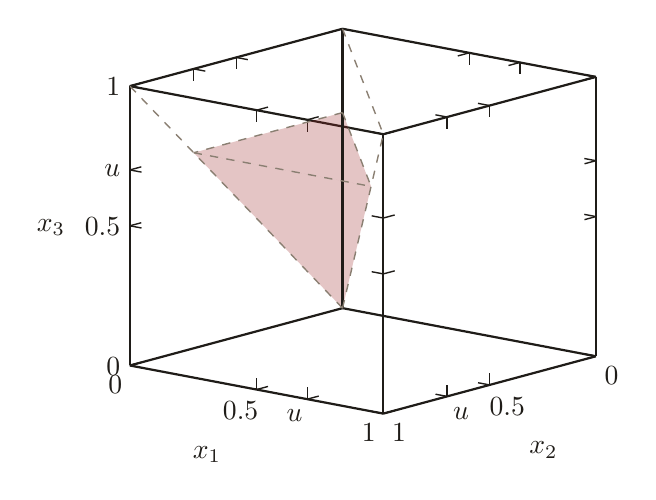
\begin{tikzpicture}
\begin{axis}[
    width=7.5cm,
    view={320}{345},
    xlabel=$x_1$,
    ylabel={$x_2$},
    zlabel={$x_3$},
    zlabel style={rotate=-90, anchor=east},
    label style={journalink},
    tick label style={journalink},
    axis line style={journalink, line width=0.8pt},
    every tick/.style={journalink, line width=0.5pt},
    enlargelimits=false,
    xmin=0, xmax=1,
    ymin=0, ymax=1,
    zmin=0, zmax=1,
    xtick={0,0.5,0.7,1}, xticklabels={0,0.5,$u$,1},
    ytick={0,0.5,0.7,1}, yticklabels={0,0.5,$u$,1},
    ztick={0,0.5,0.7,1}, zticklabels={0,0.5,$u$,1},
]

%% 四面體的四個面
\fill[journalaccent, fill opacity=0.15]
  (axis cs: 0,0,0) -- (axis cs: 0,0,0.7) -- (axis cs: 0,0.7,0.7) -- cycle;
\fill[journalaccent, fill opacity=0.15]
  (axis cs: 0,0,0) -- (axis cs: 0,0,0.7) -- (axis cs: 0.7,0.7,0.7) -- cycle;
\fill[journalaccent, fill opacity=0.15]
  (axis cs: 0,0,0) -- (axis cs: 0,0.7,0.7) -- (axis cs: 0.7,0.7,0.7) -- cycle;
\fill[journalaccent, fill opacity=0.15]
  (axis cs: 0,0,0.7) -- (axis cs: 0,0.7,0.7) -- (axis cs: 0.7,0.7,0.7) -- cycle;

%% 立方體靠前的三條稜邊
\addplot3 [journalink, line width=0.8pt, domain=0:1, samples y=1, smooth] (0, 0, x);
\addplot3 [journalink, line width=0.8pt, domain=0:1, samples y=1, smooth] (0, x, 0);
\addplot3 [journalink, line width=0.8pt, domain=0:1, samples y=1, smooth] (x, 0, 0);

%% 六條輔助虛線
\addplot3 [journalmuted, line width=0.5pt, dashed, domain=0:1, samples y=1, smooth] (x, x, x);
\addplot3 [journalmuted, line width=0.5pt, dashed, domain=0:1, samples y=1, smooth] (0, x, x);
\addplot3 [journalmuted, line width=0.5pt, dashed, domain=0:0.7, samples y=1, smooth] (x, 0.7, 0.7);
\addplot3 [journalmuted, line width=0.5pt, dashed, domain=0:0.7, samples y=1, smooth] (x, x, 0.7);
\addplot3 [journalmuted, line width=0.5pt, dashed, domain=0:1, samples y=1, smooth] (x, x, 1);
\addplot3 [journalmuted, line width=0.5pt, dashed, domain=0:0.7, samples y=1, smooth] (0, x, 0.7);

\end{axis}
\end{tikzpicture}
\end{document}
